% ============================================================
%  Full-stack E-Commerce Platform — Technical Report
%  Compiled with pdflatex (or xelatex)
% ============================================================
\documentclass[12pt,a4paper]{report}

% ---- Packages -----------------------------------------------
\usepackage[top=2.5cm, bottom=2.5cm, left=3cm, right=2.5cm, headheight=15pt]{geometry}
\usepackage{graphicx}
\usepackage[hidelinks,colorlinks=true,linkcolor=blue,urlcolor=blue,citecolor=blue]{hyperref}
\usepackage{listings}
\usepackage{xcolor}
\usepackage{enumitem}
\usepackage{booktabs}
\usepackage{array}
\usepackage{longtable}
\usepackage{fancyhdr}
\usepackage{titlesec}
\usepackage{parskip}
\usepackage{microtype}
\usepackage{tcolorbox}
\usepackage{tikz}
\usetikzlibrary{positioning}
\usepackage{amsmath}
\usepackage{amssymb}
\usepackage{float}

% ---- Page Style ---------------------------------------------
\pagestyle{fancy}
\fancyhf{}
\fancyhead[L]{\small\leftmark}
\fancyhead[R]{\small E-Commerce Platform}
\fancyfoot[C]{\thepage}
\renewcommand{\headrulewidth}{0.4pt}

% ---- Listing Styles -----------------------------------------
\definecolor{codebg}{RGB}{248,248,248}
\definecolor{codeframe}{RGB}{200,200,200}
\definecolor{commentcolor}{RGB}{0,128,0}
\definecolor{keywordcolor}{RGB}{0,0,180}
\definecolor{stringcolor}{RGB}{163,21,21}
\definecolor{numbercolor}{RGB}{100,100,100}

\lstdefinestyle{jsstyle}{
  language=Java,
  backgroundcolor=\color{codebg},
  frame=single,
  rulecolor=\color{codeframe},
  basicstyle=\ttfamily\small,
  keywordstyle=\color{keywordcolor}\bfseries,
  commentstyle=\color{commentcolor}\itshape,
  stringstyle=\color{stringcolor},
  numberstyle=\tiny\color{numbercolor},
  numbers=left,
  numbersep=8pt,
  breaklines=true,
  breakatwhitespace=true,
  tabsize=2,
  captionpos=b,
  showstringspaces=false,
  xleftmargin=15pt
}

\lstdefinestyle{jsxstyle}{
  language=HTML,
  backgroundcolor=\color{codebg},
  frame=single,
  rulecolor=\color{codeframe},
  basicstyle=\ttfamily\small,
  keywordstyle=\color{keywordcolor}\bfseries,
  commentstyle=\color{commentcolor}\itshape,
  stringstyle=\color{stringcolor},
  numberstyle=\tiny\color{numbercolor},
  numbers=left,
  numbersep=8pt,
  breaklines=true,
  breakatwhitespace=true,
  tabsize=2,
  captionpos=b,
  showstringspaces=false,
  xleftmargin=15pt
}

\lstset{style=jsstyle}

% ---- Section title formatting --------------------------------
\titleformat{\chapter}[display]
  {\normalfont\LARGE\bfseries}{\chaptername\ \thechapter}{12pt}{\LARGE}
\titlespacing*{\chapter}{0pt}{30pt}{20pt}

% ---- Colour box for "info" panels ---------------------------
\tcbuselibrary{skins,breakable}
\newtcolorbox{infobox}[1][]{
  colback=blue!5!white, colframe=blue!60!black,
  fonttitle=\bfseries, title=#1,
  breakable
}

% ============================================================
%  TITLE PAGE
% ============================================================
\begin{document}

\begin{titlepage}
  \centering
  \vspace*{2cm}

  {\Huge\bfseries MERN Stack E-Commerce Platform}\\[0.8cm]
  {\Large\itshape A Full-Stack Web Application Report}\\[2cm]

  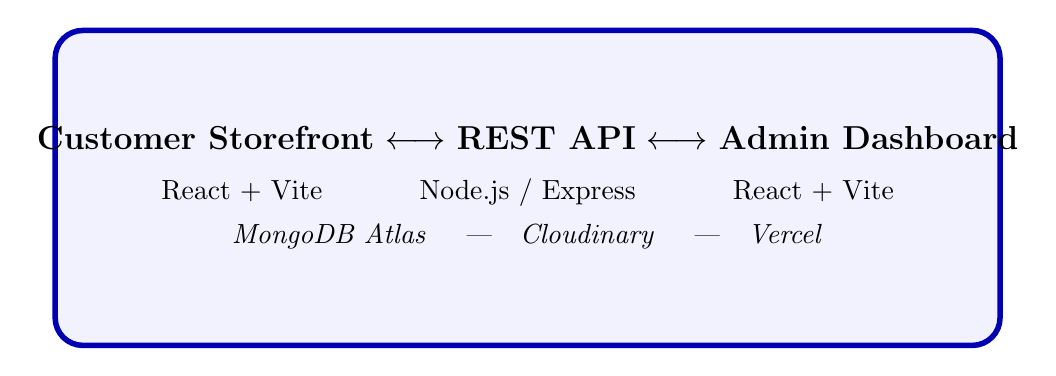
\begin{tikzpicture}
    \draw[rounded corners=10pt, line width=2pt, blue!70!black, fill=blue!5]
      (0,0) rectangle (12,4);
    \node[align=center] at (6,2) {
      \large\textbf{Customer Storefront} $\longleftrightarrow$
      \textbf{REST API} $\longleftrightarrow$
      \textbf{Admin Dashboard}\\[6pt]
      \normalsize React + Vite \hspace{1cm} Node.js / Express \hspace{1cm} React + Vite\\[4pt]
      \normalsize \textit{MongoDB Atlas \quad|\quad Cloudinary \quad|\quad Vercel}
    };
  \end{tikzpicture}

  \vspace{2cm}

  \begin{tabular}{ll}
    \textbf{Repository:} & \url{https://github.com/tashir0605/E-commerce-platform} \\[4pt]
    \textbf{Live Store:}  & \url{https://e-commerce-platform-plum.vercel.app} \\[4pt]
    \textbf{Admin Panel:} & \url{https://e-commerce-platform-admin.vercel.app} \\[4pt]
    \textbf{Backend API:} & \url{https://e-commerce-backend-teal-five.vercel.app} \\[4pt]
    \textbf{Date:}        & March 2026 \\
  \end{tabular}

  \vfill
  {\small\textit{Generated from source analysis of the complete monorepo.}}
\end{titlepage}

% ============================================================
%  ABSTRACT
% ============================================================
\chapter*{Abstract}
\addcontentsline{toc}{chapter}{Abstract}

This report presents a comprehensive technical analysis of a \textbf{MERN Stack E-Commerce Platform}
— a production-ready web application designed to facilitate online retail.
The system is structured as a monorepo containing three independently deployable sub-applications:
a customer-facing \textit{storefront}, an \textit{admin dashboard}, and a \textit{RESTful backend API}.

Built with \textbf{React}, \textbf{Node.js}, \textbf{Express.js}, and \textbf{MongoDB}, the platform supports
the complete shopping lifecycle: product browsing, size-based cart management, multi-gateway checkout
(Cash-on-Delivery, Stripe, Razorpay), and order tracking.
Cloud image storage is handled by \textbf{Cloudinary}, and all three sub-applications are deployed on
\textbf{Vercel} using a decoupled architecture.

The report covers the system architecture, technology stack, module design, data models, key algorithms,
implementation details, and directions for future improvement.
It is written to be accessible to readers with any level of technical background.

% ============================================================
%  TABLE OF CONTENTS
% ============================================================
\tableofcontents
\listoffigures
\listoftables

% ============================================================
%  CHAPTER 1 — INTRODUCTION
% ============================================================
\chapter{Introduction}

\section{Problem Statement}

Modern consumers increasingly prefer to shop online, yet building a reliable e-commerce platform is
technically challenging.
A production-grade solution must simultaneously address:

\begin{itemize}[leftmargin=*, label=\textbullet]
  \item \textbf{Product Catalogue Management} — an easy way for administrators to add, edit, and remove
        products, including multiple images per product.
  \item \textbf{Customer Experience} — an intuitive storefront with search, filtering, size selection,
        and a persistent shopping cart.
  \item \textbf{Secure Transactions} — support for multiple payment methods
        (Cash on Delivery, Stripe, Razorpay) with tamper-proof order creation.
  \item \textbf{Scalability \& Deployment} — the ability to scale each part of the system independently
        and deploy with zero downtime.
\end{itemize}

\section{Motivation}

Existing off-the-shelf solutions (e.g., Shopify) are expensive for small vendors and offer little
flexibility for custom requirements.
This project demonstrates how the \textbf{MERN stack} — a fully JavaScript, open-source technology
combination — can be used to build a feature-complete platform that is:

\begin{itemize}[leftmargin=*, label=\textbullet]
  \item \textbf{Cost-effective} — all core tools are free and open source.
  \item \textbf{Maintainable} — a single programming language (JavaScript/JSX) across all layers.
  \item \textbf{Extensible} — clearly separated modules make it easy to add new features.
  \item \textbf{Deployable} — the three sub-applications can be deployed independently on Vercel.
\end{itemize}

% ============================================================
%  CHAPTER 2 — SYSTEM OVERVIEW
% ============================================================
\chapter{System Overview}

\section{High-Level Architecture}

The platform follows a \textbf{three-tier, decoupled architecture}:

\begin{enumerate}[leftmargin=*, label=\arabic*.]
  \item \textbf{Presentation Tier} — Two React/Vite single-page applications (customer storefront and
        admin dashboard), each deployed as a separate Vercel project.
  \item \textbf{Application Tier} — A Node.js/Express RESTful API server that handles all business
        logic, authentication, and database operations.
  \item \textbf{Data Tier} — A MongoDB Atlas cloud database stores users, products, and orders.
        Cloudinary stores product images.
\end{enumerate}

\begin{figure}[H]
  \centering
  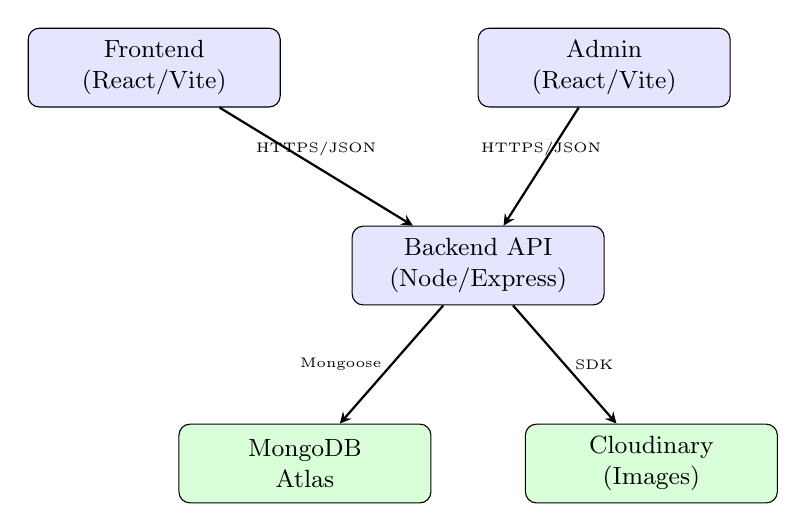
\begin{tikzpicture}[
      node distance=1.8cm,
      box/.style={draw, rounded corners=4pt, minimum width=3.2cm, minimum height=1cm,
                  align=center, fill=blue!10, font=\small},
      db/.style={draw, rounded corners=4pt, minimum width=3.2cm, minimum height=1cm,
                 align=center, fill=green!15, font=\small},
      arr/.style={->, thick, >=stealth}
    ]
    \node[box] (fe)    {Frontend\\(React/Vite)};
    \node[box] (admin) [right=2.5cm of fe] {Admin\\(React/Vite)};
    \node[box] (api)   [below=1.5cm of admin, xshift=-1.6cm] {Backend API\\(Node/Express)};
    \node[db]  (mongo) [below=1.5cm of api, xshift=-2.2cm] {MongoDB\\Atlas};
    \node[db]  (cloud) [below=1.5cm of api, xshift=2.2cm]  {Cloudinary\\(Images)};

    \draw[arr] (fe)    -- node[above,font=\tiny]{HTTPS/JSON} (api);
    \draw[arr] (admin) -- node[above,font=\tiny]{HTTPS/JSON} (api);
    \draw[arr] (api)   -- node[left,font=\tiny]{Mongoose}    (mongo);
    \draw[arr] (api)   -- node[right,font=\tiny]{SDK}         (cloud);
  \end{tikzpicture}
  \caption{High-level system architecture}
  \label{fig:arch}
\end{figure}

\section{Deployment Architecture}

Each sub-application is deployed as an independent Vercel project.
Communication between the frontend/admin and the backend uses the
\texttt{VITE\_BACKEND\_URL} environment variable, which can be switched between
\texttt{http://localhost:4000} (local) and the production URL without code changes.

\begin{table}[H]
  \centering
  \caption{Deployed Vercel Projects}
  \label{tab:deployment}
  \begin{tabular}{lll}
    \toprule
    \textbf{Project} & \textbf{Technology} & \textbf{Live URL} \\
    \midrule
    Frontend Store   & React + Vite        & \url{https://e-commerce-platform-plum.vercel.app} \\
    Admin Dashboard  & React + Vite        & \url{https://e-commerce-platform-admin.vercel.app} \\
    Backend API      & Node.js + Express   & \url{https://e-commerce-backend-teal-five.vercel.app} \\
    \bottomrule
  \end{tabular}
\end{table}

% ============================================================
%  CHAPTER 3 — TECH STACK
% ============================================================
\chapter{Tech Stack}

\section{Overview}

\begin{table}[H]
  \centering
  \caption{Technology stack with purpose and rationale}
  \label{tab:stack}
  \begin{tabular}{>{\bfseries}p{3.2cm} p{3cm} p{7cm}}
    \toprule
    Technology & Version & Purpose / Rationale \\
    \midrule
    React & 19.x & Declarative UI library with component reuse and virtual DOM rendering. \\
    Vite & 6.x & Lightning-fast dev server and build tool for React apps. \\
    Tailwind CSS & 3.x & Utility-first CSS framework that eliminates custom stylesheets. \\
    React Router & 7.x & Client-side routing for SPA navigation without full page reloads. \\
    Axios & 1.x & Promise-based HTTP client for browser \& Node.js. \\
    React Toastify & 11.x & Elegant toast notifications for success/error feedback. \\
    \midrule
    Node.js & 20+ & Non-blocking event loop ideal for I/O-heavy API servers. \\
    Express.js & 5.x & Minimal web framework for routing and middleware. \\
    Mongoose & 8.x & ODM for MongoDB; provides schema validation and query API. \\
    JSON Web Token & 9.x & Stateless authentication tokens exchanged in HTTP headers. \\
    bcrypt & 6.x & One-way password hashing with configurable cost factor. \\
    Multer & 2.x & \texttt{multipart/form-data} parser for file uploads. \\
    Cloudinary SDK & 2.x & Programmatic image upload and CDN delivery. \\
    Stripe SDK & 18.x & Stripe payment gateway integration (scaffold). \\
    Razorpay SDK & 2.x & Razorpay payment gateway integration (scaffold). \\
    validator & 13.x & Server-side input validation (email format, etc.). \\
    dotenv & 16.x & Loads \texttt{.env} variables into \texttt{process.env}. \\
    cors & 2.x & Cross-Origin Resource Sharing middleware. \\
    nodemon & 3.x & Auto-restart server on file change during development. \\
    \midrule
    MongoDB Atlas & Cloud & Managed NoSQL database with horizontal scaling. \\
    Cloudinary & Cloud & Image CDN with on-the-fly transformations. \\
    Vercel & Cloud & Zero-config deployment with global CDN edge network. \\
    \bottomrule
  \end{tabular}
\end{table}

\section{Why MERN?}

\begin{itemize}[leftmargin=*, label=\textbullet]
  \item \textbf{Single language} — JavaScript is used everywhere, reducing context switching.
  \item \textbf{JSON everywhere} — MongoDB documents, API responses, and React state all use JSON,
        making data transformation trivial.
  \item \textbf{Large ecosystem} — npm provides thousands of well-tested packages for every need.
  \item \textbf{Community \& jobs} — MERN is one of the most in-demand stacks in the industry.
\end{itemize}

% ============================================================
%  CHAPTER 4 — SYSTEM DESIGN
% ============================================================
\chapter{System Design}

\section{Monorepo Folder Structure}

The repository is organised as a \textbf{monorepo} — all three applications live in the same Git
repository but are independently deployable.

\begin{lstlisting}[caption={Top-level folder structure}, label=lst:folders, language={}]
E-commerce-platform/
|-- backend/                  # Node.js REST API
|   |-- config/               # DB & Cloudinary initialisation
|   |-- controllers/          # Route handler logic
|   |-- middleware/           # Auth & file-upload middleware
|   |-- models/               # Mongoose data schemas
|   |-- routes/               # Express router definitions
|   |-- server.js             # Application entry-point
|   `-- package.json
|
|-- frontend/                 # Customer-facing React SPA
|   `-- src/
|       |-- assets/           # Static images & asset manifest
|       |-- components/       # Reusable UI components
|       |-- context/          # React Context (global state)
|       |-- pages/            # One file per route/page
|       |-- App.jsx           # Root component & router
|       `-- main.jsx          # ReactDOM.createRoot entry
|
|-- admin/                    # Admin dashboard React SPA
|   `-- src/
|       |-- assets/
|       |-- components/       # Navbar, Sidebar, Login
|       |-- pages/            # Add, List, Orders
|       |-- App.jsx
|       `-- main.jsx
|
`-- README.md
\end{lstlisting}

\section{Backend Module Design}

\subsection{Configuration Layer (\texttt{config/})}

\begin{itemize}[leftmargin=*]
  \item \textbf{mongodb.js} — Establishes a Mongoose connection to MongoDB Atlas using the
        \texttt{MONGODB\_URI} environment variable.
  \item \textbf{cloudinary.js} — Configures the Cloudinary SDK with API credentials so product
        images can be uploaded at request time.
\end{itemize}

\subsection{Data Models (\texttt{models/})}

Three Mongoose schemas define the data layer (see Chapter~\ref{ch:impl} for schema details):

\begin{itemize}[leftmargin=*]
  \item \textbf{userModel} — Stores customers with hashed passwords and an embedded cart object.
  \item \textbf{productModel} — Stores product catalogue entries with category, size array, and
        Cloudinary image URLs.
  \item \textbf{orderModel} — Stores placed orders linked to a user ID with address, items, amount,
        payment method, and status.
\end{itemize}

\subsection{Routes \& Controllers}

Express routes map HTTP methods and paths to controller functions.
The controllers implement the actual business logic.

\begin{table}[H]
  \centering
  \caption{API endpoint summary}
  \label{tab:api}
  \begin{tabular}{llll}
    \toprule
    \textbf{Router} & \textbf{Method} & \textbf{Path} & \textbf{Protection} \\
    \midrule
    User    & POST & \texttt{/api/user/register}       & Public       \\
    User    & POST & \texttt{/api/user/login}          & Public       \\
    User    & POST & \texttt{/api/user/admin}          & Public       \\
    \midrule
    Product & POST & \texttt{/api/product/add}         & Admin token  \\
    Product & GET  & \texttt{/api/product/list}        & Public       \\
    Product & POST & \texttt{/api/product/single}      & Public       \\
    Product & POST & \texttt{/api/product/remove}      & Admin token  \\
    \midrule
    Cart    & POST & \texttt{/api/cart/add}            & User token   \\
    Cart    & POST & \texttt{/api/cart/update}         & User token   \\
    Cart    & POST & \texttt{/api/cart/get}            & User token   \\
    \midrule
    Order   & POST & \texttt{/api/order/place}         & User token   \\
    Order   & POST & \texttt{/api/order/stripe}        & User token   \\
    Order   & POST & \texttt{/api/order/razorpay}      & User token   \\
    Order   & POST & \texttt{/api/order/userorders}    & User token   \\
    Order   & POST & \texttt{/api/order/list}          & Admin token  \\
    Order   & POST & \texttt{/api/order/status}        & Admin token  \\
    \bottomrule
  \end{tabular}
\end{table}

\subsection{Middleware Layer (\texttt{middleware/})}

\begin{itemize}[leftmargin=*]
  \item \textbf{auth.js} — Extracts and verifies the JWT from the \texttt{token} request header.
        Injects \texttt{userId} into \texttt{req.body} so downstream controllers do not need to
        decode the token themselves.
  \item \textbf{adminAuth.js} — Verifies that the token payload matches the admin credentials
        string (\texttt{ADMIN\_EMAIL + ADMIN\_PASSWORD}).
  \item \textbf{multer.js} — Configures Multer disk storage so uploaded images are saved to a
        temporary path before being forwarded to Cloudinary.
\end{itemize}

\section{Frontend Module Design}

\subsection{State Management — \texttt{ShopContext}}

All global application state lives in a single React Context provider:
\texttt{src/context/ShopContext.jsx}.
It exposes:

\begin{itemize}[leftmargin=*]
  \item \textbf{products} — full product catalogue fetched once on app load.
  \item \textbf{cartItems} — a nested object \texttt{\{itemId: \{size: quantity, ...\}\}}.
  \item Helper functions: \texttt{addToCart}, \texttt{updateQuantity}, \texttt{getCartCount},
        \texttt{getCartAmount}.
  \item Auth state: \texttt{token} / \texttt{setToken} and the \texttt{backendUrl} constant.
\end{itemize}

\subsection{Pages}

\begin{table}[H]
  \centering
  \caption{Frontend page components}
  \label{tab:pages}
  \begin{tabular}{ll}
    \toprule
    \textbf{Route}           & \textbf{Component / Purpose} \\
    \midrule
    \texttt{/}               & \texttt{Home} — Hero banner, Latest Collection, Best Sellers \\
    \texttt{/collection}     & \texttt{Collection} — Filterable, sortable product grid \\
    \texttt{/product/:id}    & \texttt{Product} — Detail view with images, sizes, add-to-cart \\
    \texttt{/cart}           & \texttt{Cart} — Line items, quantity editor, cart total \\
    \texttt{/place-order}    & \texttt{PlaceOrder} — Delivery form + payment method selection \\
    \texttt{/orders}         & \texttt{Orders} — User's order history \\
    \texttt{/login}          & \texttt{Login} — Toggle-able register / login form \\
    \texttt{/about}          & \texttt{About} — Brand information \\
    \texttt{/contact}        & \texttt{Contact} — Contact form \\
    \bottomrule
  \end{tabular}
\end{table}

\subsection{Reusable Components}

\begin{itemize}[leftmargin=*]
  \item \textbf{Navbar} — Top navigation with cart badge (live count from context), search toggle,
        and profile dropdown.
  \item \textbf{SearchBar} — Animated search overlay, conditionally shown.
  \item \textbf{ProductItem} — Card for a single product (image, name, price).
  \item \textbf{BestSeller} / \textbf{LatestCollection} — Curated product grids on the home page.
  \item \textbf{RelatedProducts} — Products in the same category and subcategory.
  \item \textbf{CartTotal} — Subtotal + delivery fee summary, reused on Cart and PlaceOrder pages.
  \item \textbf{Footer} — Site links, newsletter box, social media.
  \item \textbf{OurPolicy} — Icon strip for returns, quality, and support policies.
  \item \textbf{Title} — A styled two-part heading used consistently across all pages.
\end{itemize}

\section{Admin Module Design}

The admin SPA is intentionally minimal — it authenticates against the backend's
\texttt{/api/user/admin} endpoint, stores the token in \texttt{localStorage}, and then shows one
of three pages:

\begin{itemize}[leftmargin=*]
  \item \textbf{Add} (\texttt{/Add}) — Multi-image upload form that posts to
        \texttt{/api/product/add}.
  \item \textbf{List} (\texttt{/List}) — Fetches all products and allows deletion.
  \item \textbf{Orders} (\texttt{/Orders}) — Placeholder for order management.
\end{itemize}

% ============================================================
%  CHAPTER 5 — WORKING OF THE SYSTEM
% ============================================================
\chapter{Working of the System}

\section{User Registration and Login Flow}

\begin{enumerate}[leftmargin=*, label=\arabic*.]
  \item The user visits \texttt{/login} and submits their name, email, and password.
  \item The frontend calls \texttt{POST /api/user/register} (or \texttt{login}).
  \item The backend validates the email format with the \texttt{validator} library and checks that
        the password is at least 8 characters.
  \item The password is hashed with \texttt{bcrypt} (salt rounds = 10) before storing in MongoDB.
  \item On success, the backend signs a JWT with \texttt{jwt.sign(\{id\}, JWT\_SECRET)} and returns
        the token to the client.
  \item The frontend stores the token in \texttt{localStorage} and in React context.
        Subsequent API calls include the token in the \texttt{token} HTTP header.
\end{enumerate}

\section{Product Browsing and Filtering Flow}

\begin{enumerate}[leftmargin=*, label=\arabic*.]
  \item On first load, \texttt{ShopContext} calls \texttt{GET /api/product/list}.
        All products are fetched once and cached in the \texttt{products} state array.
  \item The \texttt{Collection} page reads the full products array from context and applies
        client-side filtering by category (Men / Women / Kids), subcategory (Topwear /
        Bottomwear / Winterwear), and a search string.
  \item Sorting (low-to-high or high-to-low price) is also handled client-side with
        \texttt{Array.prototype.sort}.
  \item Clicking a product card navigates to \texttt{/product/:productId}.
        The \texttt{Product} page reads the product from the context array
        (no additional API call needed for display).
\end{enumerate}

\section{Add to Cart and Cart Management Flow}

\begin{enumerate}[leftmargin=*, label=\arabic*.]
  \item The user selects a size on the product detail page and clicks \textbf{ADD TO CART}.
  \item \texttt{addToCart(itemId, size)} in \texttt{ShopContext}:
        \begin{itemize}
          \item Validates that a size has been selected.
          \item Updates the local \texttt{cartItems} state optimistically
                (nested object: \texttt{itemId → size → quantity}).
          \item If the user is logged in, also calls \texttt{POST /api/cart/add} to persist the
                cart server-side.
        \end{itemize}
  \item On the \texttt{Cart} page, each line item is rendered with a quantity stepper.
        Changing quantity calls \texttt{updateQuantity} which updates both local state and
        \texttt{POST /api/cart/update}.
  \item The Navbar badge shows a real-time count via \texttt{getCartCount()}, which sums all
        quantities in the \texttt{cartItems} object.
\end{enumerate}

\section{Checkout and Order Placement Flow}

\begin{enumerate}[leftmargin=*, label=\arabic*.]
  \item From the Cart page the user clicks \textbf{PROCEED TO CHECKOUT} and lands on
        \texttt{/place-order}.
  \item The form collects full delivery information (name, email, street, city, state,
        zip code, country, phone).
  \item The user selects a payment method: \textbf{Stripe}, \textbf{Razorpay}, or
        \textbf{Cash on Delivery (COD)}.
  \item On submit, the frontend iterates \texttt{cartItems}, hydrates each entry with product
        data from context, and builds an \texttt{orderItems} array.
  \item For COD, the frontend calls \texttt{POST /api/order/place}.
        The backend creates an order document in MongoDB with \texttt{payment: false} and
        \texttt{status: "pending"}, then clears the user's cart.
  \item For Stripe / Razorpay, the corresponding backend endpoints
        (\texttt{/api/order/stripe}, \texttt{/api/order/razorpay}) handle payment session
        creation (scaffold implemented; full gateway integration is a future improvement).
\end{enumerate}

\section{Admin Product Management Flow}

\begin{enumerate}[leftmargin=*, label=\arabic*.]
  \item The admin logs in at the Admin Dashboard (\texttt{/}) using the email and password
        configured in the backend \texttt{.env} file.
  \item The backend's \texttt{adminLogin} controller compares credentials and returns a JWT
        if they match.
  \item The token is stored in \texttt{localStorage} and attached to every subsequent request.
  \item \textbf{Adding a product}: The admin fills in name, description, category, subcategory,
        price, sizes, bestseller flag, and up to four images.
        The form data is submitted as \texttt{multipart/form-data}.
        Multer parses the files; the controller uploads each to Cloudinary and stores the
        returned \texttt{secure\_url} values in the product document.
  \item \textbf{Listing/deleting}: The List page fetches all products and displays them in a table.
        Clicking \textbf{X} calls \texttt{POST /api/product/remove} with the product ID.
\end{enumerate}

% ============================================================
%  CHAPTER 6 — KEY ALGORITHMS / MODELS
% ============================================================
\chapter{Key Algorithms and Models}

\section{Cart Data Structure}

The cart is stored as a nested JavaScript/MongoDB object rather than an array.
This choice enables O(1) item lookup and quantity updates.

\begin{lstlisting}[caption={Cart data structure example}, label=lst:cart]
// cartData stored in MongoDB userModel.cartData field
{
  "product_id_abc": {          // product ObjectId as key
    "S":  2,                   // size "S" -> 2 units
    "M":  1
  },
  "product_id_xyz": {
    "L":  3
  }
}
\end{lstlisting}

\textbf{Key operations:}
\begin{itemize}[leftmargin=*]
  \item \textit{Add item}: \texttt{cartData[itemId][size]++} (or initialise to 1).
  \item \textit{Update quantity}: \texttt{cartData[itemId][size] = newQty}.
  \item \textit{Count}: Double loop over keys, sum all positive values.
  \item \textit{Total price}: Multiply each quantity by the corresponding product price from the
        \texttt{products} array.
\end{itemize}

\section{JWT Authentication}

JSON Web Tokens are used for stateless authentication.
A token encodes the user's MongoDB ObjectId and is signed with a secret.

\begin{lstlisting}[caption={Token creation (userController.js)}, label=lst:jwt]
import jwt from 'jsonwebtoken';

// Create a signed token containing the user's database ID
const createToken = (id) => {
  return jwt.sign({ id }, process.env.JWT_SECRET);
};
\end{lstlisting}

\begin{lstlisting}[caption={Token verification middleware (auth.js)}, label=lst:auth]
const authUser = async (req, res, next) => {
  const { token } = req.headers;  // token sent in HTTP header

  if (!token) {
    return res.json({ success: false,
                      message: 'Unauthorized access. Login Again' });
  }

  try {
    const token_decoded = jwt.verify(token, process.env.JWT_SECRET);
    req.body.userId = token_decoded.id; // inject userId for controllers
    next();
  } catch (error) {
    res.json({ success: false, message: error.message });
  }
};
\end{lstlisting}

\textbf{How it works:}
\begin{enumerate}[leftmargin=*]
  \item On login, the server signs a token with \texttt{jwt.sign} using the server's
        \texttt{JWT\_SECRET}.
  \item The client stores the token in \texttt{localStorage} and sends it in the
        \texttt{token} header on every protected request.
  \item The \texttt{authUser} middleware decodes the token; if the signature is valid,
        \texttt{req.body.userId} is populated and the request proceeds.
  \item If the token is missing or tampered with, a 200 response with
        \texttt{success: false} is returned (soft error pattern).
\end{enumerate}

\section{Password Hashing with bcrypt}

Plain-text passwords are never stored.
bcrypt uses a \textit{cost factor} (salt rounds) to make brute-force attacks computationally
expensive.

\begin{lstlisting}[caption={Password hashing on registration}, label=lst:bcrypt]
import bcrypt from 'bcrypt';

// Cost factor = 10 means 2^10 = 1024 rounds of hashing
const salt = await bcrypt.genSalt(10);
const hashedPassword = await bcrypt.hash(password, salt);

// Later, on login:
const isMatch = await bcrypt.compare(inputPassword, storedHashedPassword);
\end{lstlisting}

\section{Product Image Upload Pipeline}

\begin{enumerate}[leftmargin=*]
  \item \textbf{Multer} receives the \texttt{multipart/form-data} request and writes up to four
        image files to a local temporary directory.
  \item The \texttt{addProduct} controller filters out any undefined file slots.
  \item Each file is uploaded to Cloudinary via
        \texttt{cloudinary.uploader.upload(filePath, \{resource\_type: 'image'\})}.
  \item Cloudinary returns a \texttt{secure\_url} (HTTPS CDN URL).
  \item The array of URLs is stored in the product document's \texttt{image} field.
\end{enumerate}

\begin{lstlisting}[caption={Parallel Cloudinary upload (productController.js)}, label=lst:cloudinary]
let imagesURL = await Promise.all(
  images.map(async (item) => {
    let result = await cloudinary.uploader.upload(
      item.path,
      { resource_type: 'image' }
    );
    return result.secure_url;  // permanent CDN link
  })
);
\end{lstlisting}

\section{Client-side Filtering Algorithm}

The Collection page implements a pure client-side filter that runs every time the
filter state changes.

\begin{lstlisting}[caption={Client-side product filter (Collection.jsx — pseudocode)},
                   label=lst:filter]
// 1. Start with the full product array from context
let filtered = products;

// 2. Apply category filter (array of active categories)
if (category.length > 0)
  filtered = filtered.filter(p => category.includes(p.category));

// 3. Apply subcategory filter
if (subCategory.length > 0)
  filtered = filtered.filter(p => subCategory.includes(p.subCategory));

// 4. Apply search string
if (showSearch && search)
  filtered = filtered.filter(p =>
    p.name.toLowerCase().includes(search.toLowerCase())
  );

// 5. Sort
if (sortType === 'low-high')
  filtered.sort((a, b) => a.price - b.price);
else if (sortType === 'high-low')
  filtered.sort((a, b) => b.price - a.price);
\end{lstlisting}

% ============================================================
%  CHAPTER 7 — IMPLEMENTATION DETAILS
% ============================================================
\chapter{Implementation Details}
\label{ch:impl}

\section{Data Models}

\subsection{User Schema}

\begin{lstlisting}[caption={userModel.js}, label=lst:usermodel]
import mongoose from 'mongoose';

const userSchema = new mongoose.Schema({
  name:     { type: String, required: true },
  email:    { type: String, required: true, unique: true },
  password: { type: String, required: true },   // bcrypt hash
  cartData: { type: Object, default: {} }        // nested cart object
}, { minimize: false });  // keep empty {} in MongoDB

const userModel = mongoose.models.user
               || mongoose.model('user', userSchema);
export default userModel;
\end{lstlisting}

The \texttt{minimize: false} option is important — Mongoose's default behaviour is to remove
empty objects from documents on save; this flag keeps the \texttt{cartData: \{\}} field intact
even when the cart is empty.

\subsection{Product Schema}

\begin{lstlisting}[caption={productModel.js}, label=lst:productmodel]
const productSchema = new mongoose.Schema({
  name:        { type: String,  required: true },
  description: { type: String,  required: true },
  price:       { type: Number,  required: true },
  image:       { type: Array,   required: true }, // Cloudinary URLs
  category:    { type: String,  required: true }, // Men | Women | Kids
  subCategory: { type: String,  required: true }, // Topwear | Bottomwear | Winterwear
  sizes:       { type: Array,   required: true }, // e.g. ["S","M","L"]
  bestseller:  { type: Boolean },
  date:        { type: Number,  required: true }  // Unix timestamp
});
\end{lstlisting}

\subsection{Order Schema}

\begin{lstlisting}[caption={orderModel.js}, label=lst:ordermodel]
const orderSchema = new mongoose.Schema({
  userId:        { type: String, required: true },
  items:         { type: Array,  required: true },  // snapshot of cart items
  amount:        { type: Number, required: true },  // total in USD
  address:       { type: Object, required: true },  // delivery details
  status:        { type: String, required: true, default: 'pending' },
  paymentMethod: { type: String, required: true },  // COD | Stripe | Razorpay
  payment:       { type: Boolean, required: true, default: false },
  date:          { type: Number, required: true, default: Date.now() }
});
\end{lstlisting}

\section{Server Entry Point}

\begin{lstlisting}[caption={server.js — application bootstrap}, label=lst:server]
import express from 'express';
import cors from 'cors';
import 'dotenv/config';
import connectDB from './config/mongodb.js';
import connectCloudinary from './config/cloudinary.js';
import userRouter from './routes/userRoute.js';
import productRouter from './routes/productRoute.js';
import cartRouter from './routes/cartRoute.js';
import orderRouter from './routes/orderRoute.js';

const app = express();
const port = process.env.PORT || 4000;

connectDB();           // Mongoose connection
connectCloudinary();   // Cloudinary SDK config

app.use(express.json());
app.use(express.urlencoded({ extended: true }));
app.use(cors());       // Allow cross-origin requests from React apps

app.use('/api/user',    userRouter);
app.use('/api/product', productRouter);
app.use('/api/cart',    cartRouter);
app.use('/api/order',   orderRouter);

app.get('/', (req, res) => res.send('API WORKING'));
app.listen(port, () => console.log('Server started on PORT: ' + port));
\end{lstlisting}

\section{ShopContext — Global State}

\begin{lstlisting}[caption={ShopContext.jsx — selected excerpt}, label=lst:context]
const ShopContextProvider = (props) => {
  const backendUrl = import.meta.env.VITE_BACKEND_URL;
  const [cartItems, setCartItems] = useState({});
  const [products,  setProducts]  = useState([]);
  const [token,     setToken]     = useState('');

  // Optimistic cart update + API sync
  const addToCart = async (itemId, size) => {
    if (!size) { toast.error('Select Product Size'); return; }

    let cartData = structuredClone(cartItems); // deep-copy, no mutation
    cartData[itemId] = cartData[itemId] || {};
    cartData[itemId][size] = (cartData[itemId][size] || 0) + 1;
    setCartItems(cartData);

    if (token) {
      await axios.post(`${backendUrl}/api/cart/add`,
                       { itemId, size },
                       { headers: { token } });
    }
  };
  // ...
};
\end{lstlisting}

\section{Environment Variable Configuration}

\begin{table}[H]
  \centering
  \caption{Required environment variables}
  \label{tab:env}
  \begin{tabular}{lll}
    \toprule
    \textbf{File} & \textbf{Variable} & \textbf{Description} \\
    \midrule
    \texttt{backend/.env} & \texttt{MONGODB\_URI}          & MongoDB Atlas connection string \\
                          & \texttt{CLOUDINARY\_NAME}      & Cloudinary cloud name \\
                          & \texttt{CLOUDINARY\_API\_KEY}  & Cloudinary API key \\
                          & \texttt{CLOUDINARY\_SECRET\_KEY} & Cloudinary API secret \\
                          & \texttt{JWT\_SECRET}           & Secret for JWT signing \\
                          & \texttt{ADMIN\_EMAIL}          & Admin login email \\
                          & \texttt{ADMIN\_PASSWORD}       & Admin login password \\
    \midrule
    \texttt{frontend/.env} & \texttt{VITE\_BACKEND\_URL}  & Backend base URL \\
    \texttt{admin/.env}    & \texttt{VITE\_BACKEND\_URL}  & Backend base URL \\
    \bottomrule
  \end{tabular}
\end{table}

% ============================================================
%  CHAPTER 8 — RESULTS / OUTPUT
% ============================================================
\chapter{Results and Output}

\section{Key User Flows}

\subsection{Home Page}
The home page greets visitors with a full-width \textbf{Hero} section containing a call-to-action
button.
Below it, the \textbf{Latest Collection} grid renders the 10 most recently added products, and the
\textbf{Best Sellers} section highlights products marked \texttt{bestseller: true} in the database.
The \textbf{Our Policy} strip communicates exchange, quality, and 24/7 support policies using icons.

\subsection{Product Detail Page}
The product detail page shows:
\begin{itemize}[leftmargin=*]
  \item A thumbnail strip + main image viewer (clicking a thumbnail updates the main image).
  \item A static 4-star rating and review count.
  \item Price, description, and a size selector that highlights the chosen option.
  \item An \textbf{ADD TO CART} button that is only active after a size is selected.
  \item A \textbf{Related Products} row filtered to the same category and subcategory.
\end{itemize}

\subsection{Checkout Page}
The checkout page is split two columns:
\begin{itemize}[leftmargin=*]
  \item \textit{Left} — Delivery information form (8 required fields).
  \item \textit{Right} — Cart total summary and payment method selector
        (Stripe, Razorpay, or Cash on Delivery).
\end{itemize}

\subsection{Admin Add Product}
The Add Product form in the admin dashboard allows uploading up to 4 images by clicking
placeholder boxes, filling in all product metadata, toggling sizes and the bestseller flag,
and submitting via a single \textbf{ADD} button.

\subsection{Admin Product List}
The List page renders a table of all products with their thumbnail, name, category, and price.
Each row has a delete button that removes the product from MongoDB and refreshes the list.

\section{Sample API Responses}

\begin{lstlisting}[caption={Successful product list response}, label=lst:resp1, language={}]
{
  "success": true,
  "products": [
    {
      "_id": "664a1b2c3d4e5f6789abcdef",
      "name": "Classic Oxford Shirt",
      "description": "A timeless Oxford shirt for formal occasions.",
      "price": 49,
      "image": [
        "https://res.cloudinary.com/demo/image/upload/v1/shirt_1.jpg",
        "https://res.cloudinary.com/demo/image/upload/v1/shirt_2.jpg"
      ],
      "category": "Men",
      "subCategory": "Topwear",
      "sizes": ["S", "M", "L", "XL"],
      "bestseller": true,
      "date": 1716432000000
    }
  ]
}
\end{lstlisting}

\begin{lstlisting}[caption={Successful user login response}, label=lst:resp2, language={}]
{
  "success": true,
  "token": "eyJhbGciOiJIUzI1NiIsInR5cCI6IkpXVCJ9.eyJpZCI..."
}
\end{lstlisting}

\begin{lstlisting}[caption={Successful order placement response}, label=lst:resp3, language={}]
{
  "success": true,
  "message": "Order placed successfully"
}
\end{lstlisting}

% ============================================================
%  CHAPTER 9 — CHALLENGES FACED
% ============================================================
\chapter{Challenges Faced}

\section{CORS Configuration in a Decoupled Architecture}

\textbf{Problem:} Three separate origins (two Vercel frontend domains + localhost during
development) need to communicate with the same backend.
A browser's Same-Origin Policy blocks cross-origin requests by default.

\textbf{Solution:} The \texttt{cors} middleware is applied globally to all Express routes
with default settings that allow all origins.
In production, this should be tightened to an explicit origin whitelist for security.

\section{File Upload with Multipart Forms to a Serverless Backend}

\textbf{Problem:} Vercel's serverless functions have ephemeral file systems.
Multer's disk storage writes to \texttt{/tmp}, which is not persistent between invocations.

\textbf{Solution:} Images are uploaded to Cloudinary immediately after Multer writes them
to the temporary path.
Only the Cloudinary CDN URLs (not the files themselves) are stored in MongoDB.
This pattern eliminates any dependency on local disk persistence.

\section{Case-Sensitive Imports on Linux-Based CI/CD}

\textbf{Problem:} Developers on macOS (case-insensitive file system) could write
\texttt{import Sidebar from './components/sidebar'} and it would work locally but fail on
Vercel's Linux runners, which enforce exact capitalisation.

\textbf{Solution:} The README explicitly documents strict naming conventions:
component filenames and import paths must match exactly (PascalCase for component files).

\section{Cart Persistence for Guest vs. Logged-In Users}

\textbf{Problem:} A guest user who adds items to the cart and then logs in would lose their
cart, or the cart state could conflict between local state and the server-side cart.

\textbf{Solution:} The cart state is maintained in React context (in-memory) for guest users.
When a user logs in, \texttt{getUserCart} is called to hydrate the context from the
server-side cart stored in MongoDB, effectively merging the sessions.

\section{Mongoose \texttt{minimize: false} — Empty Cart Bug}

\textbf{Problem:} After placing an order, the cart is cleared by setting
\texttt{cartData: \{\}}.
Mongoose's default \texttt{minimize: true} option strips empty objects before saving,
so the \texttt{cartData} field would disappear entirely from the document, causing
\texttt{TypeError: Cannot read properties of undefined} on the next cart read.

\textbf{Solution:} The User schema is instantiated with \texttt{\{minimize: false\}},
which preserves empty objects in the database.

\section{Admin Authentication Without a Dedicated Admin User Collection}

\textbf{Problem:} A full role-based access control system is complex to implement and
outside the scope of a single-developer project.

\textbf{Solution:} A lightweight approach is used: the admin's email and password are
stored only in the backend \texttt{.env} file.
On login, the credentials are compared directly.
The JWT payload is the concatenated string \texttt{ADMIN\_EMAIL + ADMIN\_PASSWORD},
which the \texttt{adminAuth} middleware validates.

% ============================================================
%  CHAPTER 10 — FUTURE IMPROVEMENTS
% ============================================================
\chapter{Future Improvements}

\begin{enumerate}[leftmargin=*, label=\arabic*.]
  \item \textbf{Complete Stripe and Razorpay Integration} — The backend scaffolding for payment
        gateways already exists; the next step is to implement webhook handlers for payment
        confirmation and update order \texttt{payment} status accordingly.

  \item \textbf{Order Management in Admin Panel} — The \texttt{Orders.jsx} admin page is currently
        empty.
        It should fetch all orders via \texttt{POST /api/order/list} and allow the admin to
        update statuses (e.g., ``Processing'', ``Shipped'', ``Delivered'').

  \item \textbf{User Order History on the Storefront} — The \texttt{/orders} frontend page is
        scaffold-only.
        It should call \texttt{POST /api/order/userorders} and display a list of past orders
        with status tracking.

  \item \textbf{Product Search with MongoDB Text Index} — Currently all filtering is client-side.
        For large catalogues, adding a MongoDB text index on \texttt{name} and \texttt{description}
        fields and implementing server-side search would dramatically reduce the payload.

  \item \textbf{Product Reviews and Ratings} — The static 4-star display and ``Reviews (122)''
        label should be replaced with a real review system: a \texttt{reviewModel},
        a \texttt{POST /api/product/review} endpoint, and an aggregated star rating.

  \item \textbf{Inventory / Stock Management} — Add a \texttt{stock} field per size variant so
        the system can prevent overselling and display ``Out of Stock'' badges.

  \item \textbf{Email Notifications} — Integrate a transactional email service (e.g., SendGrid,
        Resend) to send order confirmation and shipping update emails.

  \item \textbf{Admin RBAC} — Replace the single hard-coded admin with a role-based access control
        system that supports multiple admins and permission levels
        (e.g., inventory manager vs. super admin).

  \item \textbf{Image Optimisation} — Use Cloudinary's transformation API to serve
        appropriately-sized images (e.g., thumbnails vs. full-size) and convert to WebP format
        for improved Core Web Vitals.

  \item \textbf{Unit and Integration Tests} — Add a test suite (e.g., Jest + Supertest for the
        backend, React Testing Library for the frontend) to prevent regressions as the codebase
        grows.

  \item \textbf{CORS Hardening} — Replace the wildcard \texttt{cors()} call with an explicit
        \texttt{origin} whitelist containing only the two production Vercel domains.

  \item \textbf{Pagination} — Implement cursor-based or page-number pagination on the
        \texttt{/api/product/list} endpoint to support large catalogues without transferring
        the entire database on every page load.
\end{enumerate}

% ============================================================
%  CHAPTER 11 — CONCLUSION
% ============================================================
\chapter{Conclusion}

This report has presented a detailed technical analysis of a full-stack MERN e-commerce platform.
The project demonstrates that a small team — or a single developer — can build a production-capable
online shopping system using freely available, open-source technologies.

\textbf{Key achievements:}
\begin{itemize}[leftmargin=*, label=\checkmark]
  \item A \textbf{decoupled three-tier architecture} that allows the frontend, admin, and API to be
        scaled and deployed independently on Vercel.
  \item \textbf{Secure authentication} using JWTs and bcrypt-hashed passwords.
  \item A \textbf{clean API surface} with 14 endpoints covering users, products, cart, and orders.
  \item \textbf{Cloud-native image handling} via Cloudinary, eliminating disk storage concerns on
        serverless infrastructure.
  \item A \textbf{React Context-based global state} that keeps cart and auth state synchronised
        across the entire SPA without the complexity of Redux.
  \item An \textbf{optimistic UI} pattern in the cart: the interface updates instantly while the
        API call proceeds in the background, resulting in a snappy user experience.
\end{itemize}

The platform is a solid foundation.
The most impactful next steps — completing the payment gateway integration, implementing the order
management UI, and adding product reviews — would turn it into a fully feature-complete retail system
ready for real customers.

\vspace{1cm}
\begin{tcolorbox}[colback=blue!5, colframe=blue!60!black, title=Quick Reference]
  \begin{tabular}{ll}
    \textbf{Live Store:}     & \url{https://e-commerce-platform-plum.vercel.app} \\
    \textbf{Admin Panel:}    & \url{https://e-commerce-platform-admin.vercel.app} \\
    \textbf{Backend API:}    & \url{https://e-commerce-backend-teal-five.vercel.app} \\
    \textbf{Repository:}     & \url{https://github.com/tashir0605/E-commerce-platform} \\
  \end{tabular}
\end{tcolorbox}

% ============================================================
%  END OF DOCUMENT
% ============================================================
\end{document}
